%!TEX root = ../main.tex

\section{Germanium}
\label{sec:germanium}

Bei der ersten untersuchten Probe handelt es sich um einen konventionellen Germanium-
Halbleiter der mittels elektrolytischer Goldkontakte und -drähte an die Messapperatur
angeschlossen ist. Das Germanium-Plättchen hat, wie in \autoref{fig:germanium} 
gezeigt, die Ausmaße H$\times$W$\times$L = $\SI{1}{\milli\meter}\times\SI{10}{\milli
\meter}\times\SI{19}{\milli\meter}$. Im Folgenden sollen nun einige elektronische
Eigenschaften in Abhängigkeit der Temperatur des Halbleiters diskutiert werden.

\begin{figure}
	\centering
	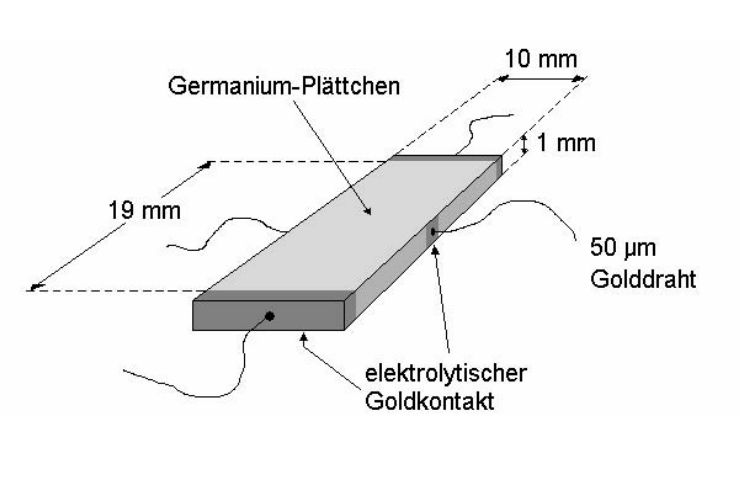
\includegraphics[width=0.6\textwidth]{./fig/germanium.png}
	\caption{Schematische Darstellung der Germanium Probe, deren Ausmaß und 
	zugehöriger Elektronik. Abbildung entnommen aus Laborhandbuch \cite{Manual}}.
	\label{fig:germanium}
\end{figure}

\subsection{Leitfähigkeit und Hallkoeffizient}
\label{ssec:leitfähigkeit}

Die Leitfähigkeit $\sigma$ sowie der Hallkoeffizient $R_\text{Hall}$ werden wie in 
\autoref{chap:theory} dargestellt berechnet. Dabei ergeben sich über verschiedene
Temperaturen die in \autoref{fig:measurement_A} und \autoref{fig:logarithmic_A} 
gezeigten Verläufe. Die gemessenen Spannungswerte, aus denen diese Größen berechnet 
sind sind dem Protokoll in \autoref{chap:germanium-data} beigefügt.

\begin{figure}[H]
	\centering
	\begin{subfigure}[h]{0.45\linewidth}
	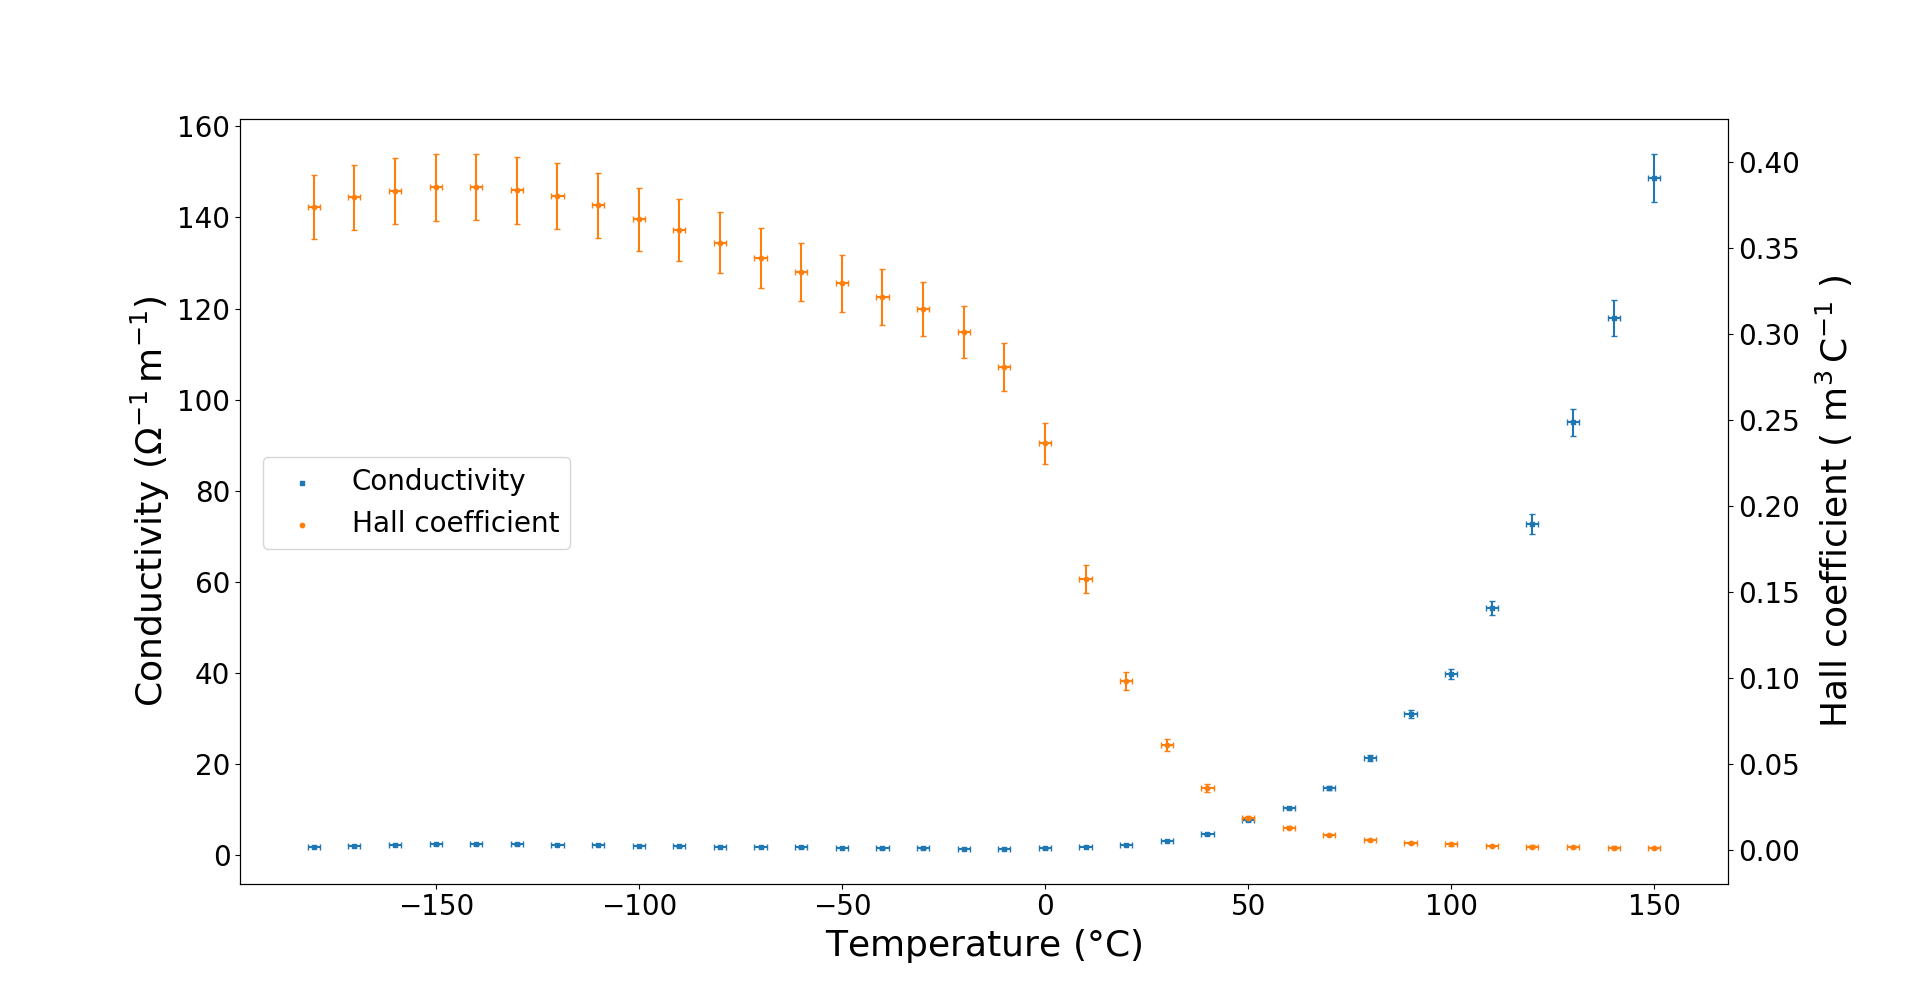
\includegraphics[height=4.2cm]{./fig/probe_A_measurement.png}
	\caption{\textbf{Messwerte Probe A}\label{fig:measurement_A}}
	\end{subfigure}
	\hfill
	\begin{subfigure}[h]{0.45\linewidth}
	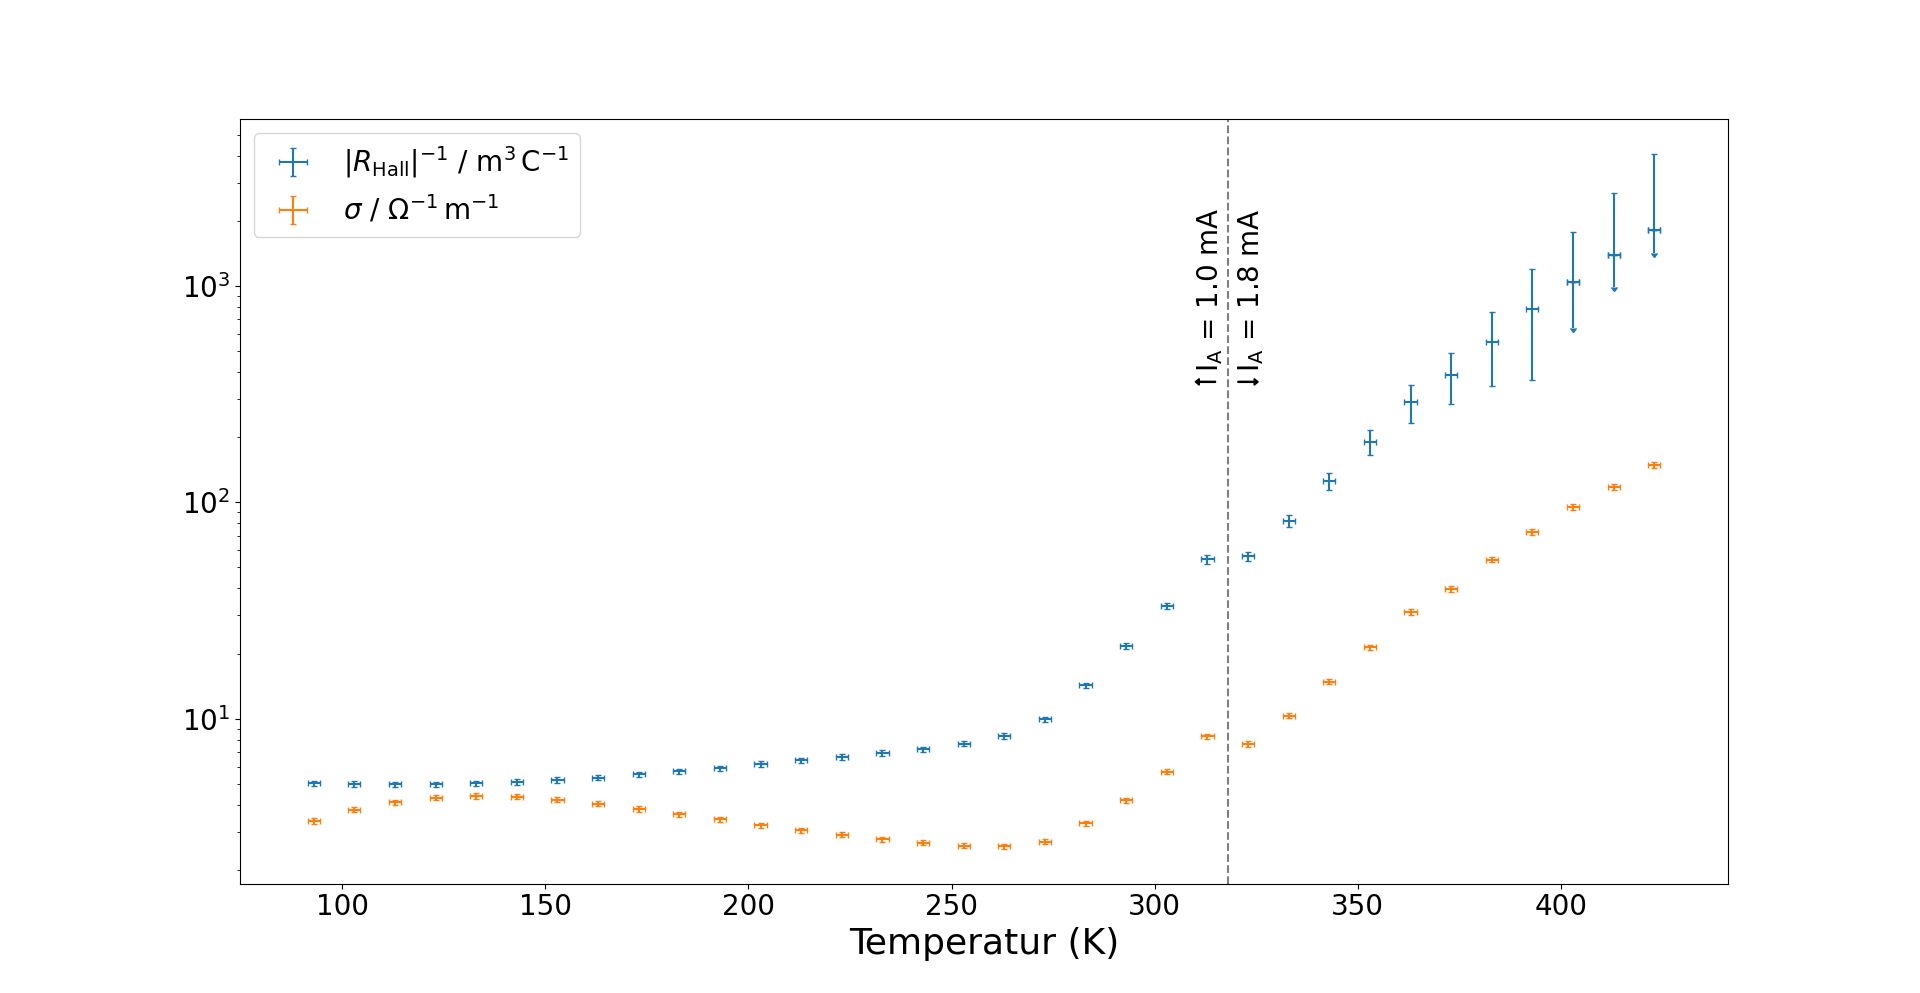
\includegraphics[height=4.2cm]{./fig/probe_A_combined_plot.png}
	\caption{\textbf{kombinierte logarithmische Darstellung}
\label{fig:logarithmic_A}}
	\end{subfigure}
	\caption*{\textbf{a)} Erkennbar ist die exponentielle Abhängigkeit der 
Leitfähigkeit $\sigma$ von der Temperatur $T$. Während der Hallkoeffizient für tiefe
Temperaturen betragsmäßig groß ist nimmt der Effekt für große Temperaturen ab. 
\textbf{b)} Logarithmische Darstellung der Messwerte. Der extrinsiche Bereich 
befindet sich um \SI{200}{\kelvin}, der intrinsische oberhalb von \SI{350}{\kelvin} 
\label{measurements_A}}
\end{figure}

In den obigen Schaubildern sind qualitativ unterschiedliche Verhalten beider 
Messgrößen gegenüber der Temperatur zu erkennen. Zwar ist der Hallkoeffizient über
den gesamten Messbereich hinweg negativ und die Ladungsträger damit Elektronen jedoch
ändert sich die Ladungsträgerkonzentration und Beweglichkeit der Ladungsträger 
deutlich beim Abkühlen des Halbleiters. Diese qualitativen Abhängigkeiten werden in 
den folgenden Unterabschnitten genauer behandelt.

\subsection{Extrinsicher- und intrinsischer Leitbereich}
\label{ssec:extrinsic-intrinsic}

Hierzu wird die Beweglichkeit der Ladungsträger untersucht. Im extrinsischen 
Leitbereich entspricht diese dem Produkt aus Leitfähigkeit und  Betrag des 
Hallkoeffizienten

\begin{equation}
\label{eq:mobility}
	\mu = \sigma\,|R_\text{Hall}|
\end{equation}

Die Abhängigkeit der Elektronen(-löcher)mobilität ist dargestellt in 
\autoref{fig:mobility}. Gut zu erkennen sind zwei lineare Bereiche in dem doppelt-
logarithmischen Plot. Hierbei handelt es sich um den ex- und intrinsischen Bereich,
die sich durch Anzahl und Beschaffenheit der anwesenden Ladungsträger wie in
\autoref{chap:theory} diskutiert unterscheiden. Eine qualitative Analyse befindet,
dass sich die beiden Bereiche über folgende Temperaturdomänen erstrecken

\begin{align*}
	\SI{173}{\kelvin}\;\leq\;&T_\text{ext}\;\leq\;\SI{253}{\kelvin} \\
	&T_\text{int}\;\geq\;\SI{343}{\kelvin}
\end{align*}

\begin{figure}
	\centering
	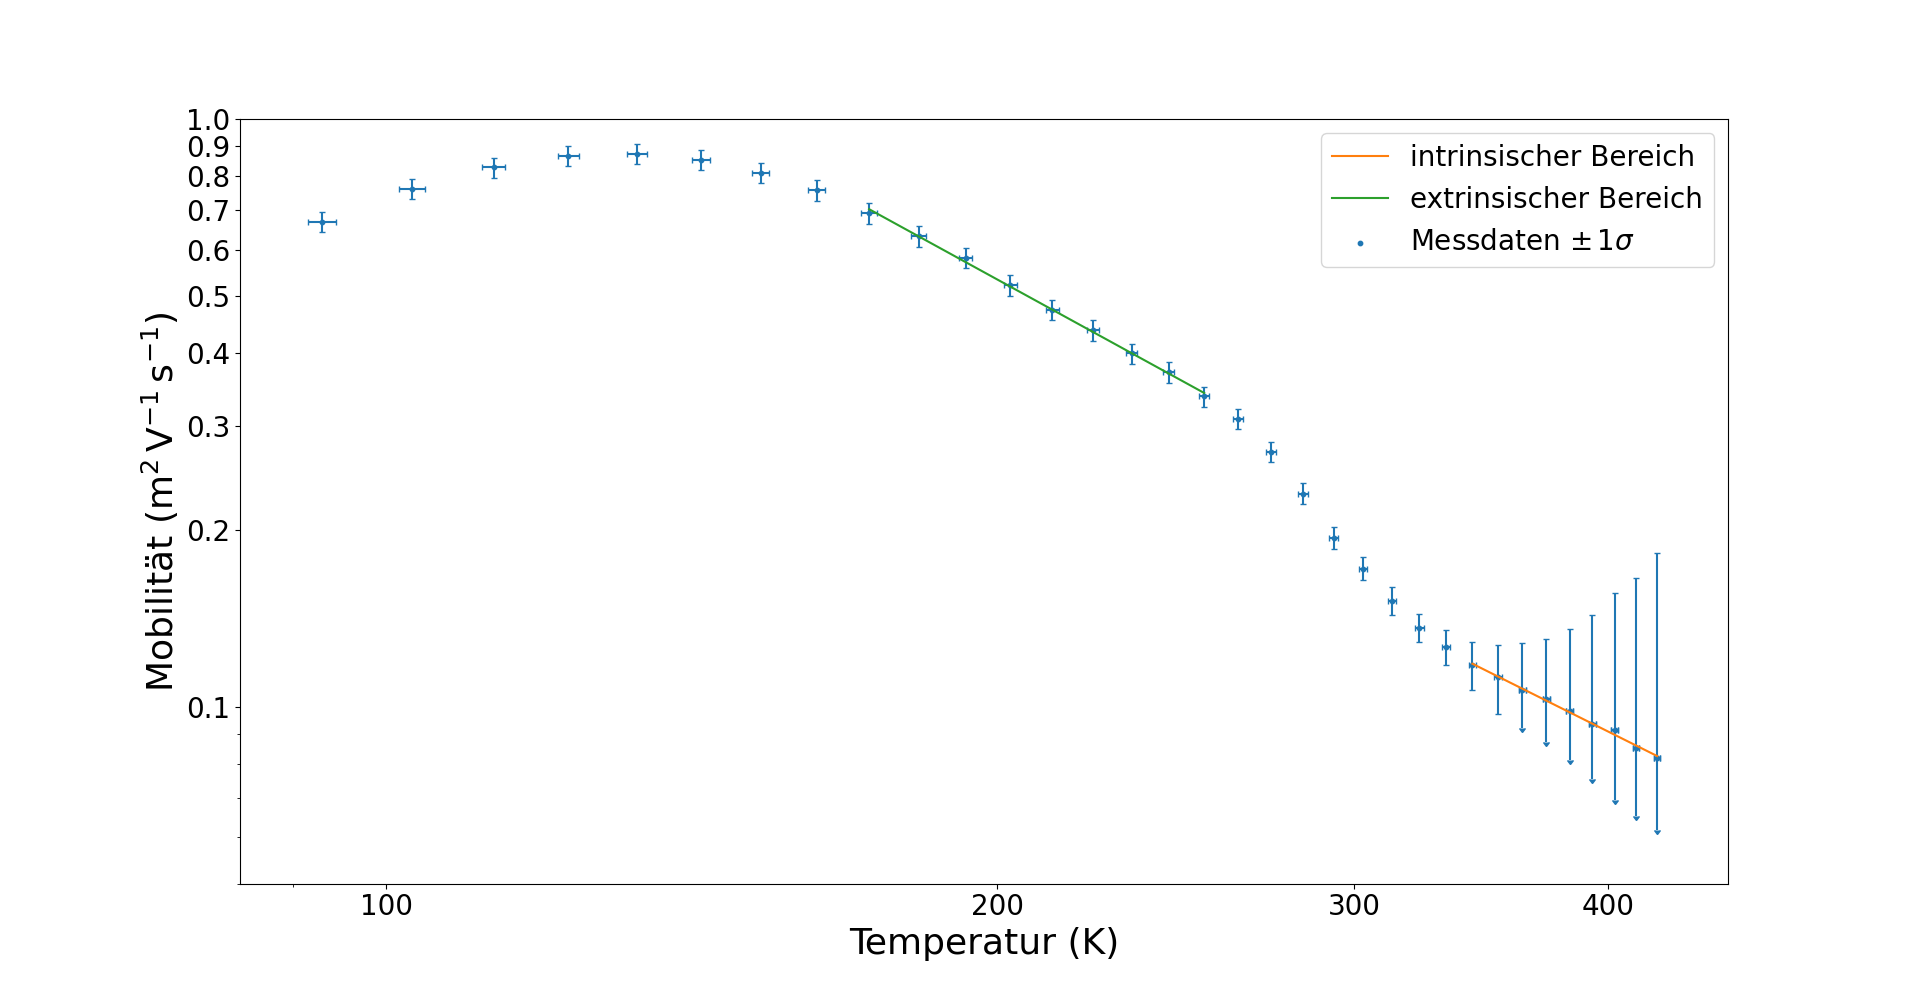
\includegraphics[width=1.0\textwidth]{./fig/mobility.png}
	\caption{Ladungsträgerbeweglichkeit über Temperatur}
	\label{fig:mobility}
\end{figure}

\subsection{Ladungsträgerkonzentration und Bandlücke}
\label{ssec:charge-carrier-concentration}

Die Ladungsträgerkonzentration im intrinsischen Bereich $n_i$ lässt sich mittels der 
in \autoref{chap:theory} und  \cite{Manual} präsentierten Zusammenhänge leicht aus 
dem Hallkoeffizienten herleiten.

\begin{equation}
\label{eq:ccc}
	n_i = \frac{1}{|e|R_\text{Hall}}\,\frac{1-b(T)}{1+b(T)},
\end{equation}

wobei $b(T)$ das Verhältnis der Beweglichkeiten von Elektronen und Elektronenlöchern
angibt $b(T):=\frac{\mu_e(T)}{\mu_h(T)}$. Dieses wird im Laborhandbuch angegeben mit
$b(T) = 1.24553\,+\,1.07\times10^{-3}\,T$. Damit errechnen sich Werte für die
Ladungsträgerkonzentration, die in \autoref{fig:charge-carrier-concentration} gezeigt
sind.

Weiterhin lässt sich aus dem Verlauf der Ladungsträgerkonzentration mittels der 
\textit{Arrhenius}-Darstellung die Bandlücke $E_\text{gap}$ des Halbleiters 
bei $T=\SI{0}{\kelvin}$ bestimmen. Dabei wird \autoref{eq:arrhenius} über die 
reziproke Temperatur aufgetragen. Im damit gewonnenen Schaubild ist also eine lineare
Abhägigkeit der Messpunkte von $T^{-1}$ zu erwarten. Eine lineare Regression findet 
eine Gerade mit Steigung $-\frac{E_\text{gap}(T=0)}{2k_B}$ und Y-Achsenabschnitt
$\log(A')$.

\begin{equation}
\label{eq:arrhenius}
	\log\left( \frac{n_i}{T^\frac{2}{3}}\right) = \log(A') - \frac{E_\text{Gap}(T=0)}{2k_B\,T}
\end{equation}

Die Arrhenius-Darstellung ist in \autoref{fig:arrhenius} gezeigt. Dabei ergibt die 
oben präsentierte Analyse die Fitparameter in \autoref{eq:fitparams_A}. 

\begin{align}
\label{eq:fitparams_A}
	\log(A') &= 41.1\pm2.6 \\
	E_\text{Gap}(T=0) &= \SI{0.881\pm0.046}{\electronvolt} 
\end{align}

Im letzten Teil der Analyse der Germanium Probe wird nun die Bandlücke sowie
Ladungsträgerkonzentration des Germaniumplättchens bei Raumtemperatur 
(\SI{300}{\kelvin}) bestimmt. Hierzu ist erneut das Laborhandbuch \cite{Manual} sowie
die in \autoref{chap:theory} dargestellten Zusammenhänge hilfreich. Die Bandlücke 
des Germaniumhalbleiters ist schwach Temperaturabhängig. Es gilt:

\begin{align*}
E_\text{Gap}(T) &= E_\text{Gap}(T=0) - \SI{4e-4}{\electronvolt\per\kelvin}\;T \\
	E_\text{Gap}(\SI{300}{\kelvin}) &= \SI{0.761\pm0.046}{\electronvolt}
\end{align*}

Mit diesem Wissen und \autoref{eq:arrhenius} lässt sich die Konzentration der
Ladungsträger bei einer beliebigen Temperatur berechnen als

\begin{align*}
\label{eq:charge-carrier-concentration}
	n_i(T) &= A'\,T^{\frac{2}{3}}\;e^{-\frac{E_\text{Gap}(T)}{2k_B\,T}}, \\
	n_i(\SI{300}{\kelvin}) &= \SI{1.306\pm0.12e13}{\per\centi\meter\cubed}
\end{align*}

Die gefundenen Werte weichen von Literaturwerten des Laborhandbuchs ab 
($E_\text{Gap, Lit.}(T=\SI{300}{\kelvin}=\SI{0.66}{\electronvolt}$, 
$n_{i,\text{Lit.}}=\SI{2.4e13}{\per\centi\meter\cubed}$). Die Messungenauigkeiten
alleine können diese relativ hohen Abweichungen alleine vollständig erklären. Im 
Messaufbau selber müssen folglich unbehandelte Systematiken auftauchen, die in dieser
Analyse nicht diskutiert werden. Nichtsdestotrotz kann  eine qualitative
Übereinstimmung der Daten mit der Theorie gezeigt werden.

\begin{figure}
	\centering
	\begin{subfigure}[h]{0.45\linewidth}
	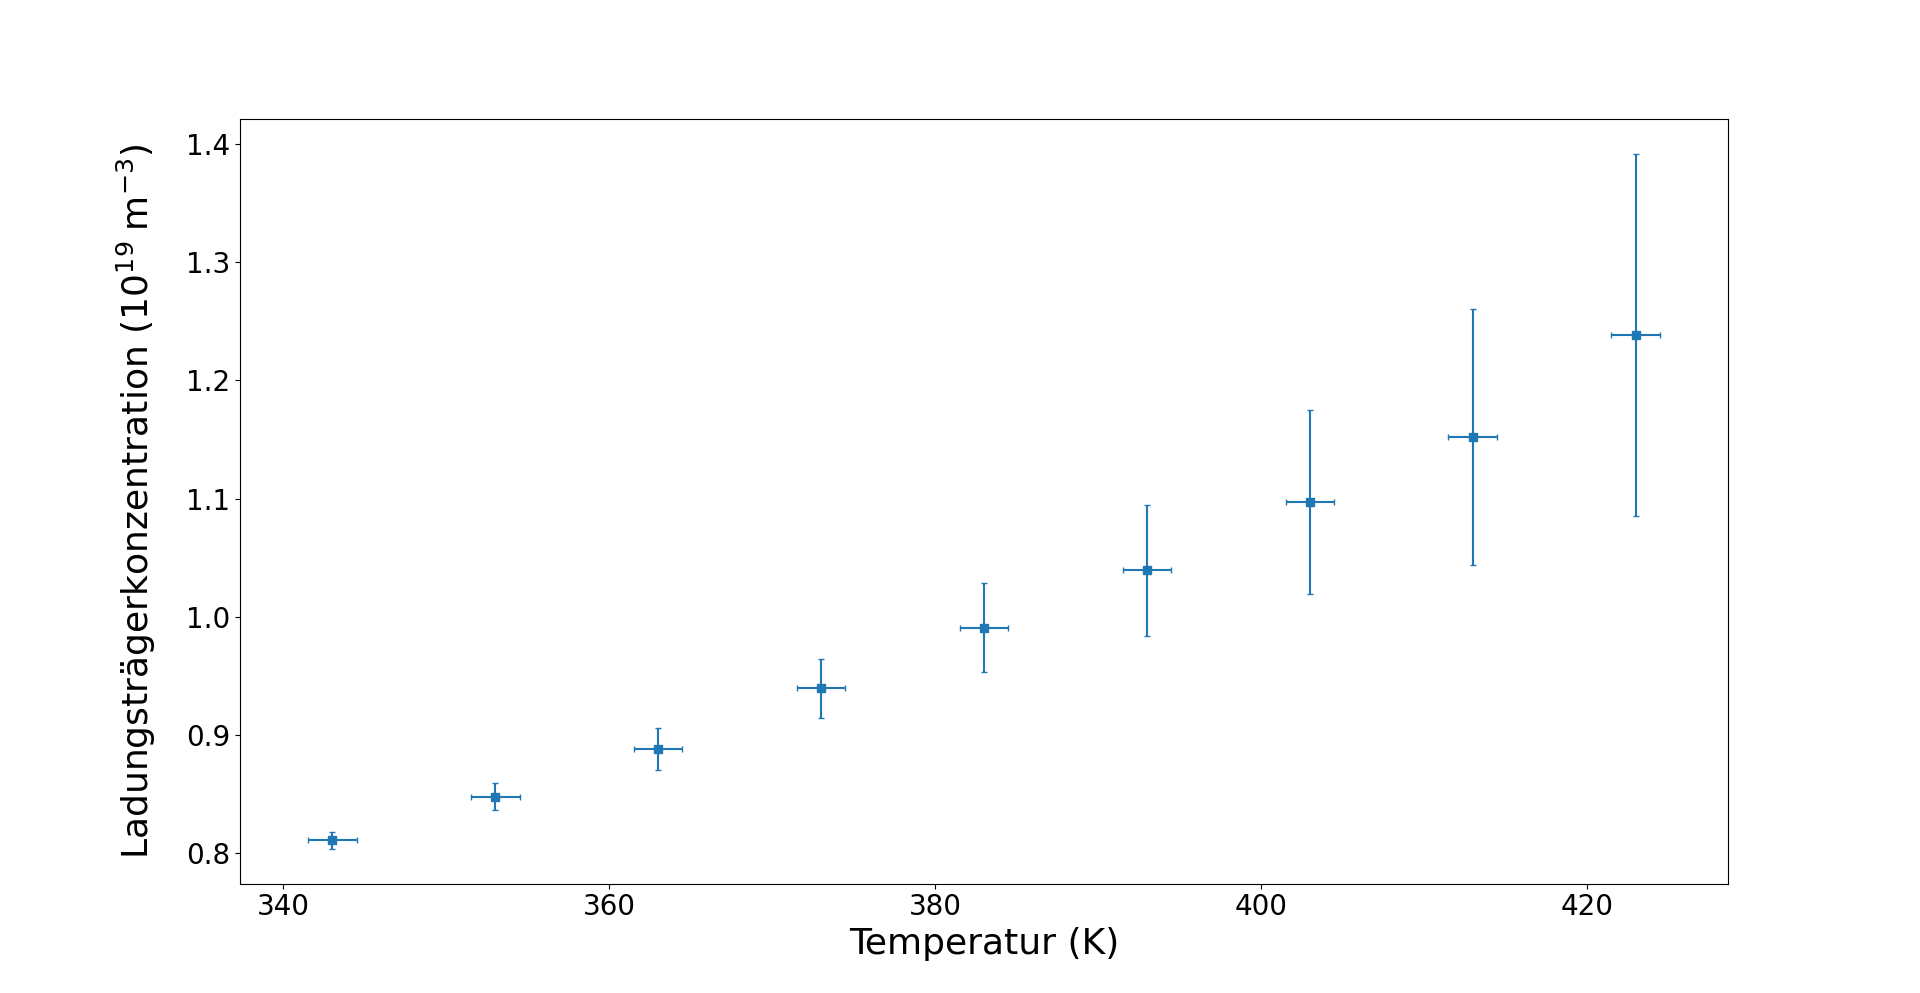
\includegraphics[height=4.2cm]{./fig/charge_carrier_concentration.png}
	\caption{\textbf{Ladungsträgerkonzentration im intrinsischen Bereich}\label{fig:charge-carrier-concentration}}
	\end{subfigure}
	\hfill
	\begin{subfigure}[h]{0.45\linewidth}
	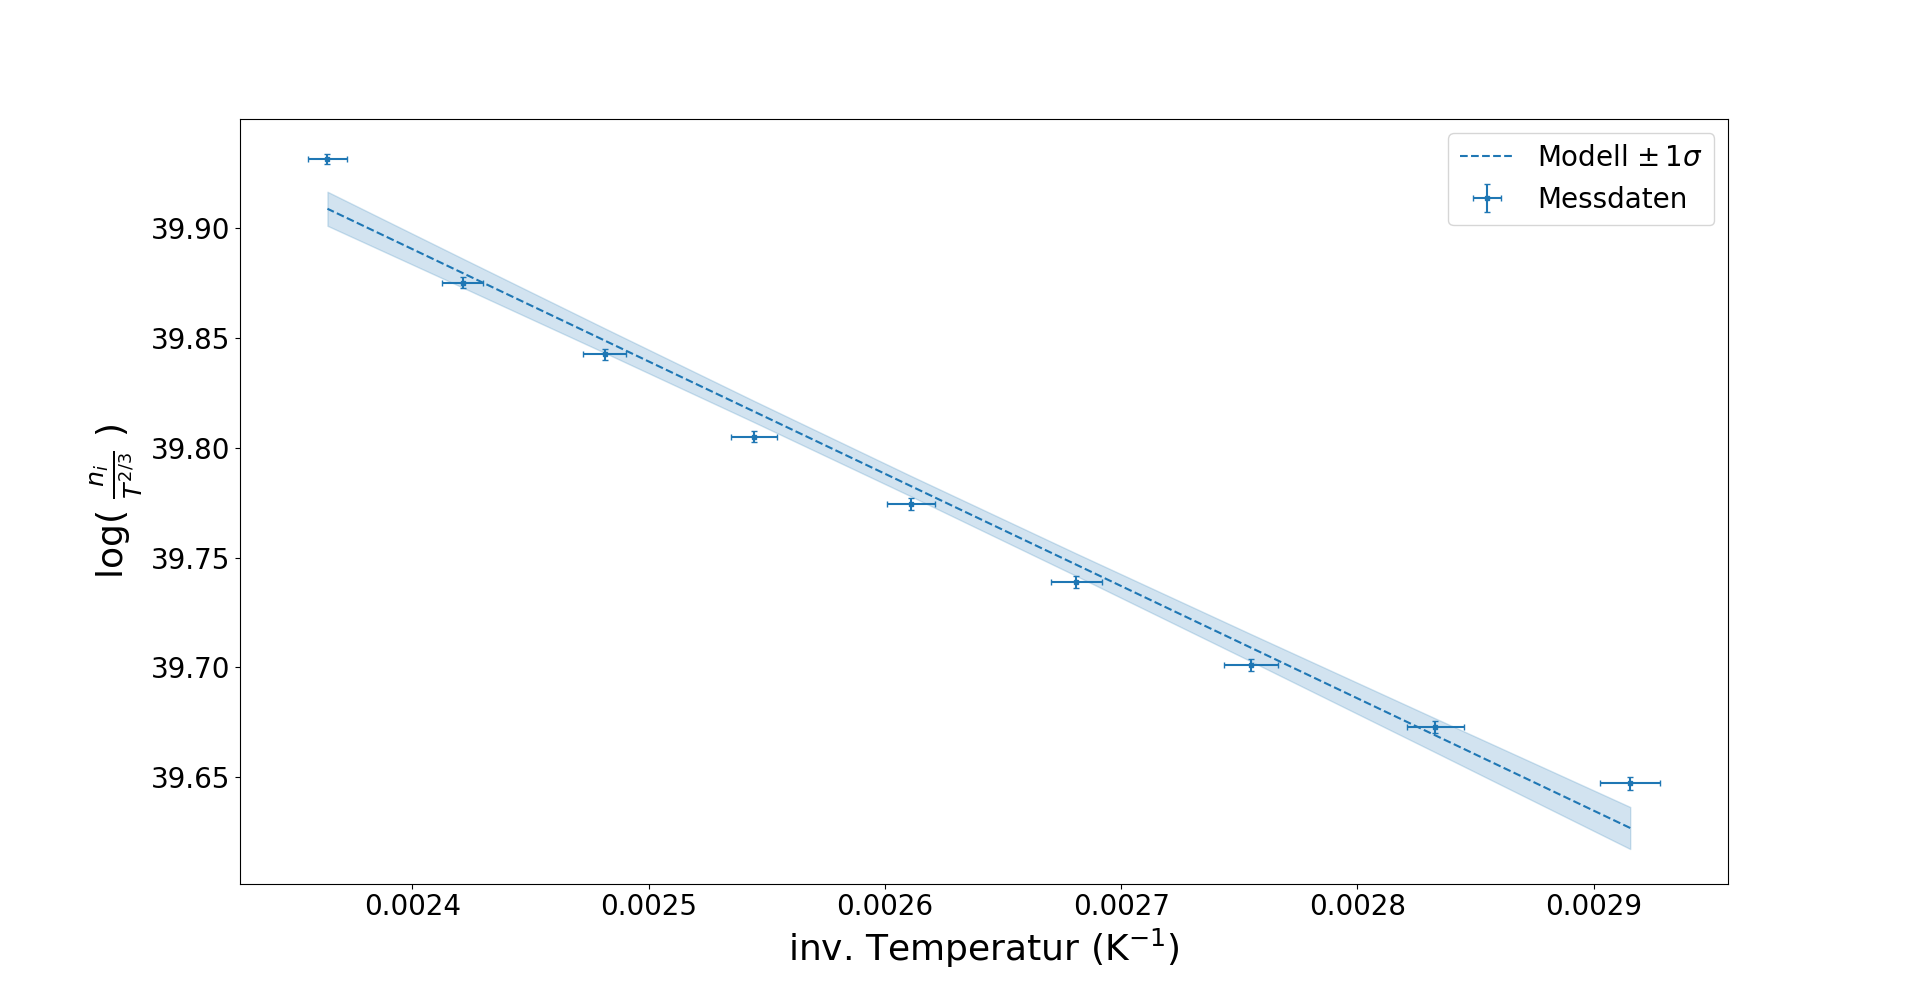
\includegraphics[height=4.2cm]{./fig/arrhenius_plot.png}
	\caption{\textbf{Arrhenius Darstellung}\label{fig:arrhenius}}
	\end{subfigure}
	\caption*{\textbf{a)} Die Ladungsträgerkonzentration wächst durch thermische 
	Anregungen bei steigenden Temperaturen. \textbf{b)} Arrhenius Darstellung zur
	Berechnung der Bandlücke des Halbleiters. \label{fig:analysis_A}}
\end{figure}
